% Chapter 1

\chapter{Ensemble Statistics}
\label{Chapter4}

\section{Ensemble Spread}

The ensemble spread is an important statistic for ensemble based DA systems as it gives us the general scale of the background error covariances. This in comparison with the observation error tells us how much weight will be given to observations at a given location and time. Figure \ref{fig:hsvarseries} shows a timeseries of the ensemble variance in Hs from the run beginning 10$^\text{th}$ March, alongside the ensemble mean. This is shown both for the buoy location and for a spatial average over the entire domain.

As with the observations, we see that the variance is a strong function of the mean. The variance at the buoy location peaks just before the peak in the mean, and drops back to lower value as the mean reaches its peak. This means that observations from just before the peak will be given higher weighting in the DA than most, as the background error is high compared to the observation error. Conversely, observations taken during and shortly after the peak will be given lower weighting as the observation error at this point is high while the background error is low.

From the plot of spatial mean, we see an overall upward trend in ensemble variance over time, as is to be expected in any forecast. This means that observations closer to the end of the assimilation window will usually be given higher weighting than those taken earlier, since the background error will be greater in comparison to the observation error.

\begin{figure}
\centering
\begin{subfigure}{.49\textwidth}
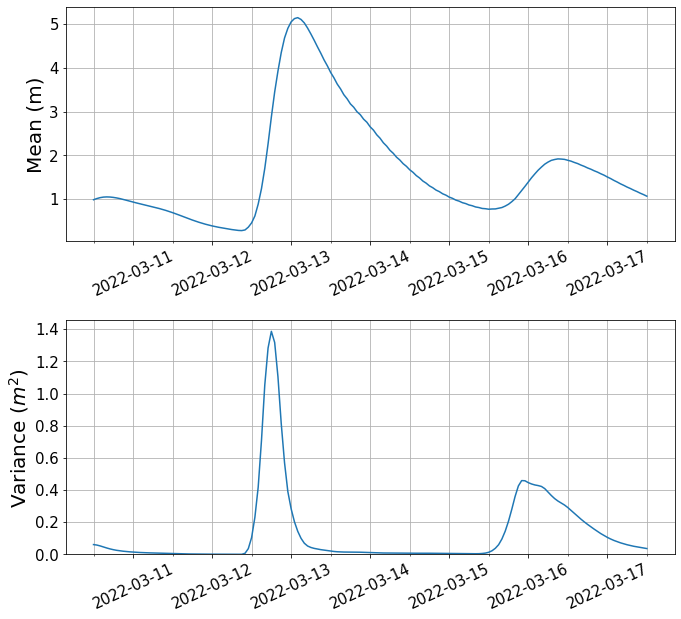
\includegraphics[width = \textwidth]{figures/buoyhsvar}
\end{subfigure}
\begin{subfigure}{.49\textwidth}
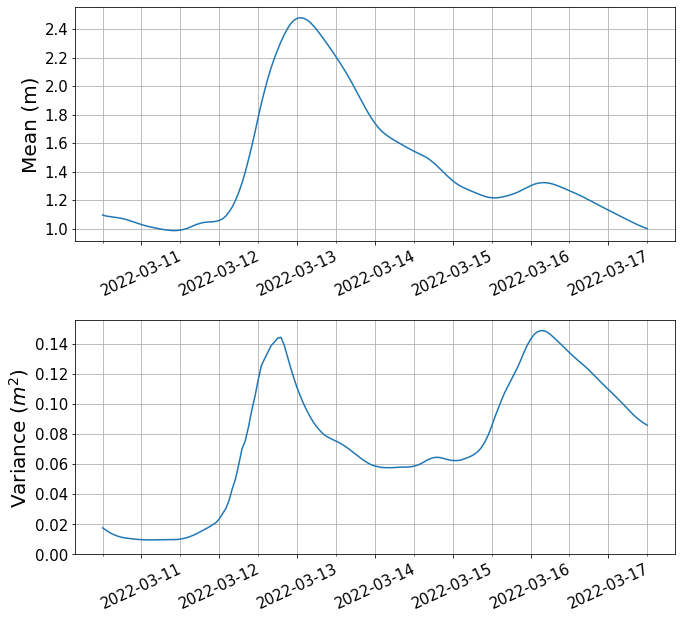
\includegraphics[width = \textwidth]{figures/meanhsvar}
\end{subfigure}
\caption{\textbf{Left:} Timeseries of Hs ensemble mean (top) and variance (bottom) from the buoy location. Data is taken from the run beginning $10^\text{th}$ March 2022. \textbf{Right:} Same as left but a spatial average is taken over the entire domain before taking the ensemble mean and variance.}
\label{fig:hsvarseries}
\end{figure}

Figure \ref{fig:t01varseries} Shows the same as figure \ref{fig:hsvarseries} but for Tm01. From the buoy timeseries, we see a sharp peak in variance just before the peak in Tm01, similar to what we saw for Hs. We also see that the swell event is preceded by a dip in Tm01 ensemble mean, which also corresponds with a peak in variance just before. (from this we may hypothesise that variance is highest when the variable in question is changing quickly - test) Since Tm01 observation errors also scale with Tm01, this means that observations from from shortly before the event will be given higher weighting and observations taken during and shortly after will be given lower weighting. The spatial mean plot shows a very strong upward trend in variance with leadtime, so as with Hs, Tm01 observations will tend to be given higher weighting if they are closer to the end of the assimilation window. (Tm02 has very similar characteristics to Tm01 and is not discussed further here.)

\begin{figure}
\centering
\begin{subfigure}{.49\textwidth}
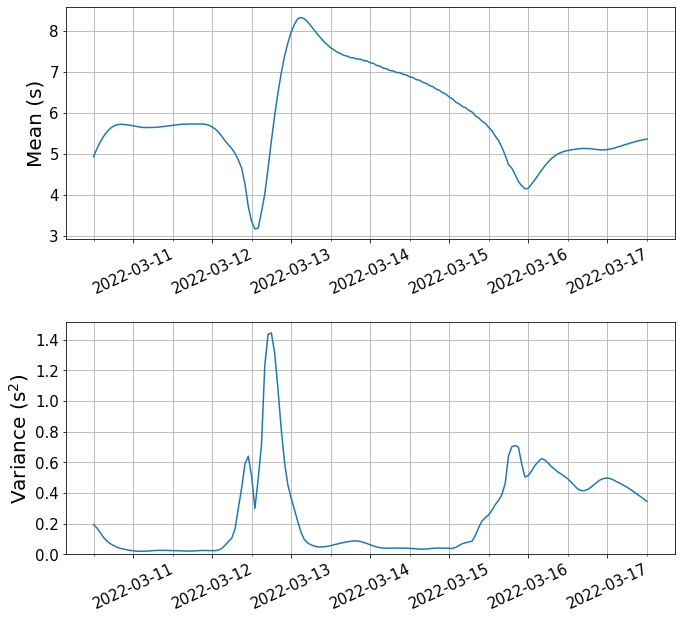
\includegraphics[width = \textwidth]{figures/buoyt01var}
\end{subfigure}
\begin{subfigure}{.49\textwidth}
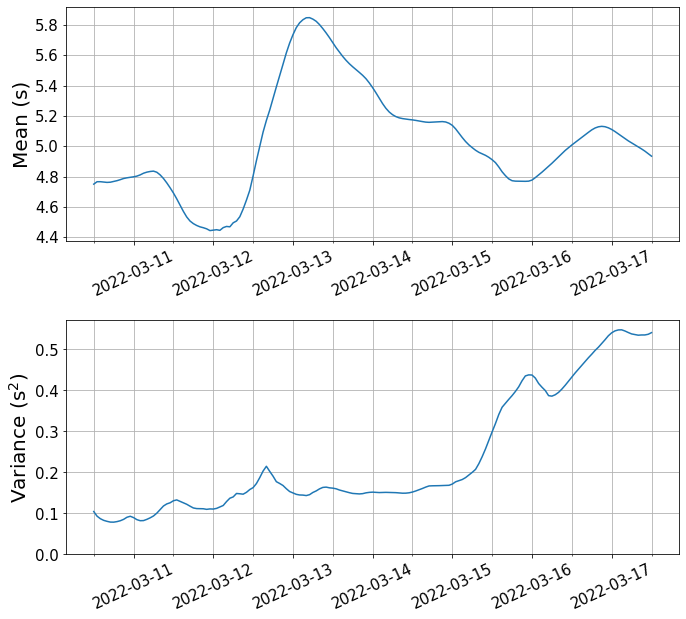
\includegraphics[width = \textwidth]{figures/meant01var}
\end{subfigure}
\caption{\textbf{Left:} Timeseries of Tm01 ensemble mean (top) and variance (bottom) from the buoy location. Data is taken from the run beginning $10^\text{th}$ March 2022. \textbf{Right:} Same as left but a spatial average is taken over the entire domain before taking the ensemble mean and variance.}
\label{fig:t01varseries}
\end{figure}

\section{Covariances}

\subsection{Spatial Covariances}

\subsection{Cross Covariances in Time}

\subsection{Cross Covariances Between Variables}

